\chapter{量子物理导论}\label{ch:b1:quantum-introduction}

用紫外光照射干净的金属，电子会立即飞出，其能量取决于光的颜色，而与光的亮度完全无关；
改用红光照射，无论灯多亮，都没有电子逸出。
让电子一个一个地通过双缝，每个电子都落在屏上一个确定的位置——
这些落点累积到数千个之后，
便形成波的条纹。这两个事实都与前二十九章的物理不相容。
本章介绍与之相容的思想：光以量子的形式出现，即光子；
物质具有波长；
传播的是\omterm{def:b1:wave-propagation:signal}{振幅}，其模方为概率；
位置与动量不能同时精确确定；
束缚粒子只能取某些特定的能量——
正因如此，原子才有确定的大小，光谱才有谱线，
而直径仅几纳米的半导体颗粒
会发出由其直径决定颜色的光。

\section{光子}

\begin{theorem}[普朗克–爱因斯坦关系]\label{thm:b1:quantum-introduction:photon}
\index{光子}\index{普朗克常量}
频率为 $\nu$、波长为 $\lambda$ 的光仅以量子的形式与物质交换能量，
这些量子即\emph{光子}，其能量与动量分别为
\[
E = h\nu = \frac{hc}{\lambda} , \qquad p = \frac{h}{\lambda} = \frac{E}{c} ,
\]
其中\emph{\omterm{thm:b1:quantum-introduction:photon}{普朗克常量}} $h = \qty{6.626e-34}{J.s}$（$\hbar = h/2\pi =
\qty{1.055e-34}{J.s}$）。常用关系为 $hc = \qty{1240}{eV.nm}$——
一个波长为 \qty{620}{nm} 的光子携带 \qty{2}{eV} 的能量。
\end{theorem}
\admitted

\begin{proposition}[光电效应]\label{prop:b1:quantum-introduction:photoelectric}
\index{光电效应}\index{逸出功}\index{遏止电压}
照射到一种\emph{\omterm{prop:b1:quantum-introduction:photoelectric}{逸出功}}为 $W$ 的金属上的光（即
金属中束缚最弱的电子的束缚能，约为几个 eV），会打出电子，
其最大\omterm{thm:b1:work-and-energy:ke}{动能}为
\[
E_{k,\max} = h\nu - W ,
\]
因此仅当频率高于\emph{阈值} $\nu_0 = W/h$ 时，\omterm{prop:b1:quantum-introduction:photoelectric}{光电效应}才会发生，且几乎瞬时发生，
电子的能量与光强无关；光强决定的是
每秒逸出电子的\emph{数目}。使电流恰好为零的\emph{\omterm{prop:b1:quantum-introduction:photoelectric}{遏止电压}}
$V_s$ 测得 $E_{k,\max} = eV_s$，而以 $V_s$ 对 $\nu$ 作图，
得到斜率为 $h/e$ 的直线——
密立根正是由此测得 $h$。
\end{proposition}

\begin{proof}
每个光子被一个电子吸收，该电子获得的能量至多为 $h\nu - W$；
若光是波，则能量会连续传给每一个电子，
能量将随光强增大，而弱光需要数小时才能
在一个原子上积累足够的 $W$（见\cref{pb:b1:quantum-introduction:1}）——
这些现象均未被观察到。爱因斯坦的解释（1905 年）
在本阶段作为定律不加证明地承认。
\end{proof}

\begin{omfigure}
\begin{tikzpicture}[font=\small, x=1cm, y=1cm, >=Stealth]
  % apparatus
  \draw[fill=omExo!25, draw=omExo, thick] (-2.2,-1.2) rectangle (-1.7,1.2); \node[font=\footnotesize] at (-1.95,-1.5) {阴极};
  \draw[omThm, thick] (1.7,-1.2) -- (1.7,1.2); \node[font=\footnotesize] at (1.7,-1.5) {阳极};
  \foreach \y in {0.6,0.2,-0.2} \draw[omProp, ->, decorate, decoration={snake, amplitude=1.5pt, segment length=4pt, post length=3pt}] (-3.8,\y+0.6) -- (-2.25,\y);
  \node[omProp, font=\footnotesize] at (-3.6,1.55) {光，$\nu$};
  \foreach \y in {0.7,0,-0.7} \draw[omDef, ->] (-1.65,\y) -- (0.4,\y);
  \node[omDef, font=\footnotesize] at (0,1.0) {$E_k \leq h\nu - W$};
  \draw (-1.95,-1.2) -- (-1.95,-2.2) -- (1.7,-2.2) -- (1.7,-1.2);
  \draw[fill=white] (-0.6,-2.45) rectangle (0.4,-1.95); \node[font=\footnotesize] at (-0.1,-2.2) {$V_s$};
  \node[font=\footnotesize] at (-0.1,-2.75) {阳极接 $-V_s$：电流恰好为零};
\end{tikzpicture}\hfill
\begin{tikzpicture}
\begin{axis}[omaxis, axis x line=bottom, axis y line=left, width=7.4cm, height=5.4cm,
    xlabel={$\nu$ ($10^{14}$ Hz)}, ylabel={$V_s$ (V)},
    xlabel style={at={(axis description cs:1.0,0.0)}, anchor=north east, yshift=-10pt},
    xmin=0, xmax=12.5, ymin=0, ymax=3, xtick={2,4,...,12}, ytick={1,2,3}, samples=2, clip=false]
  \addplot[omDef, thick, domain=5.32:12] {0.4136*x-2.2};
  \addplot[only marks, mark=*, mark size=1.6pt, omThm] coordinates {(6,0.30) (7,0.69) (8,1.13) (9,1.50) (11,2.36)};
  \addplot[omDef, dashed, thin, domain=3.6:5.32] {0.4136*x-2.2};
  \node[font=\footnotesize, omDef, anchor=east] at (axis cs:3.4,-0.6) {截距 $-W/e$};
  \node[font=\footnotesize, anchor=south] at (axis cs:5.32,0.05) {$\nu_0$};
  \node[font=\footnotesize, omDef, anchor=west] at (axis cs:8.4,0.9) {斜率 $h/e$};
\end{axis}
\end{tikzpicture}

{\small 左：光电池——光将电子从阴极中打出；
恰好足以使电子停止运动的反向\omterm{def:b1:dc-circuits:voltage}{电压} $V_s$ 即可测出其最大能量。
右：对于每种金属，\omterm{prop:b1:quantum-introduction:photoelectric}{遏止电压}与频率的关系都是斜率为 $h/e$ 的直线；
截距给出\omterm{prop:b1:quantum-introduction:photoelectric}{逸出功}，
阈值给出最小频率。}
\end{omfigure}

\begin{example}[数量级]\label{ex:b1:quantum-introduction:orders}
一个可见光光子：\qty{2}{eV}；一个波长为 \qty{0.1}{nm} 的 X 射线光子：\qty{12}{keV}；
一个频率为 \qty{100}{MHz} 的无线电光子：\qty{4e-7}{eV}。一台功率为 \qty{1}{mW} 的红色\omterm{rem:b1:quantum-introduction:rest}{激光器}每秒发射 $10^{-3}/(3.1 \times 10^{-19}) = 3 \times 10^{15}$ 个光子；
一根在 \qty{100}{MHz} 下接收 \qty{1}{pW} 功率的无线电天线，每秒接收 $10^{13}$
个光子——数量如此之多，每个又如此之小，以至于对任何用途而言，
波动描述都是精确的；相比之下，人眼可以察觉
由一百个光子组成的闪光。光的量子性在光子数少或能量高时显现：
光电池、X 射线探测器，以及
微弱照片的颗粒感。
%
\end{example}

\begin{remark}[康普顿散射]\label{rem:b1:quantum-introduction:compton}
\index{康普顿散射}
光子与自由电子碰撞时，像台球一样传递动量：
其波长增大 $\Delta\lambda = \frac{h}{m_ec}(1 -
\cos\theta)$，其中 $h/m_ec = \qty{2.43}{pm}$（在本阶段不加证明地承认——这是相对论性碰撞，
属于本科二年级内容）。对可见光而言，该效应不可见（$\Delta\lambda/\lambda \sim 10^{-5}$），
而对 X 射线则是 $20\%$ 的效应；1923 年，
正是这一实验使怀疑者信服光子携带动量 $h/\lambda$。
\end{remark}

\section{物质波}

\begin{theorem}[德布罗意]\label{thm:b1:quantum-introduction:debroglie}
\index{德布罗意波长}\index{物质波}
动量为 $p$ 的粒子以波动形式传播，其波长为
\[
\lambda = \frac{h}{p} ,
\]
并相应地表现出衍射和干涉：电子在
晶体上（戴维孙与革末，1927 年）、经双缝（约恩松，1961 年）、
中子、原子，以及由 60 个碳原子组成的分子。对于一个电子，
经\omterm{def:b1:dc-circuits:voltage}{电压} $U$ 加速后，$\lambda = h/\sqrt{2m_eeU} = \qty{1.23}{nm}/\sqrt{U/\unit{V}}$。
\end{theorem}
\admitted

\begin{example}[为何从未观察到它]\label{ex:b1:quantum-introduction:wavelengths}
能量为 \qty{100}{eV} 的电子：$\lambda = \qty{0.12}{nm}$，与
晶体中原子的间距相当，因此会发生衍射，这也是电子
\omterm{def:b1:optical-instruments:microscope}{显微镜}得以实现的原因。热中子（\qty{0.025}{eV}）的波长为 \qty{0.18}{nm}。一个
质量为 \qty{1}{g}、速率为 \qty{1}{m/s} 的小球：$\lambda = \qty{7e-31}{m}$，
比原子核小 $10^{20}$ 倍：任何狭缝或晶体都无法使它发生衍射。
物质的波动性是普遍的；其波长使它
仅对光和慢速粒子才可见。
\end{example}

\begin{proposition}[单个粒子构成条纹]\label{prop:b1:quantum-introduction:buildup}
\index{波粒二象性}
一次一个地让电子通过双缝（外村，1989 年），每个电子
在屏幕上留下一个亮点，其位置无法预先确定；
这些亮点累积成双缝干涉图样，该图样属于一列
波长为 $h/p$ 的波。关闭一条狭缝会抹去条纹——图样
并非电子彼此干涉的结果，而是由
每个电子的波同时穿过两条狭缝所致。探测粒子经过的是哪一条狭缝，
同样会抹去条纹。
\end{proposition}
\admitted

\begin{omfigure}
\begin{tikzpicture}[font=\small, x=1cm, y=1cm]
  \begin{scope}
    \draw (-3.2,0) rectangle (3.2,1.3);
    \foreach \x/\y in {-0.42/0.13, -0.48/1.04, 1.15/0.56, 0.55/0.59, 0.60/0.75, -0.69/0.53, -0.22/0.63, 0.11/0.48, 0.98/1.01, 0.53/1.14, 0.15/0.07, 0.79/0.66, 0.45/0.89, -1.25/0.96, 0.00/0.26, -3.08/0.35, -0.16/1.17, 1.20/1.23, -0.61/0.47, -1.22/0.48, -1.91/0.66, 0.03/1.05, 1.17/0.88, -0.07/0.05, 0.75/0.82, -1.25/0.73, 1.23/0.86, 0.11/0.61, 3.06/1.17, -1.18/1.06, -0.46/0.38, 0.07/0.28, 0.15/0.50, 0.53/0.52, 0.65/0.06, 1.12/0.55, 1.07/1.16, 1.06/1.19, -1.17/0.38, -0.73/0.35, -0.04/1.16, -1.62/0.13, -0.53/0.79, 0.05/0.33, 0.53/1.17, 0.62/0.79, 1.14/0.27, -1.20/0.73, -0.49/1.03, 0.11/0.51, 0.64/0.71, -0.48/0.84, -0.07/0.33, -0.17/0.18, 0.07/0.10, 0.07/0.12, -0.78/1.19, -0.05/1.20, 0.04/0.43, 1.15/1.12} \fill[omDef] (\x,\y) circle (1.1pt);
    \node[font=\footnotesize] at (0,-0.35) {$60$ 个电子};
  \end{scope}
  \begin{scope}[yshift=-2.4cm]
    \draw (-3.2,0) rectangle (3.2,1.3);
    \foreach \x/\y in {-0.42/0.13, -0.48/1.04, 1.15/0.56, 0.55/0.59, 0.60/0.75, -0.69/0.53, -0.22/0.63, 0.11/0.48, 0.98/1.01, 0.53/1.14, 0.15/0.07, 0.79/0.66, 0.45/0.89, -1.25/0.96, 0.00/0.26, -3.08/0.35, -0.16/1.17, 1.20/1.23, -0.61/0.47, -1.22/0.48, -1.91/0.66, 0.03/1.05, 1.17/0.88, -0.07/0.05, 0.75/0.82, -1.25/0.73, 1.23/0.86, 0.11/0.61, 3.06/1.17, -1.18/1.06, -0.46/0.38, 0.07/0.28, 0.15/0.50, 0.53/0.52, 0.65/0.06, 1.12/0.55, 1.07/1.16, 1.06/1.19, -1.17/0.38, -0.73/0.35, -0.04/1.16, -1.62/0.13, -0.53/0.79, 0.05/0.33, 0.53/1.17, 0.62/0.79, 1.14/0.27, -1.20/0.73, -0.49/1.03, 0.11/0.51, 0.64/0.71, -0.48/0.84, -0.07/0.33, -0.17/0.18, 0.07/0.10, 0.07/0.12, -0.78/1.19, -0.05/1.20, 0.04/0.43, 1.15/1.120} \fill[omDef] (\x,\y) circle (1.1pt);
    \node[font=\footnotesize] at (0,-0.35) {$600$ 个电子};
  \end{scope}
  \begin{scope}[yshift=-4.6cm]
    \draw (-3.2,0) rectangle (3.2,1.3);
    \foreach \x/\y in {-0.02/0.94, 1.23/0.49, -1.77/0.11, 0.08/1.17, 0.58/0.98, -0.45/0.37, -1.29/0.96, -0.08/0.50, 0.27/1.07, -0.57/0.51, -0.57/0.28, -0.12/0.06, -0.00/0.62, 0.20/0.90, -0.01/0.81, -0.08/1.16, 0.57/0.90, -1.18/0.87, 0.47/0.79, 0.15/0.87, -0.77/1.01, -0.58/0.94, 0.06/1.13, 0.67/0.72, 1.29/0.61, 0.75/0.17, 1.23/0.09, -0.76/1.08, -1.29/0.68, -0.14/0.59, -1.13/0.63, 0.56/0.63, 0.13/0.95, 0.61/0.32, 0.05/0.24, -1.19/1.21, -0.68/0.95, 0.08/0.95, -1.25/0.14, -0.00/0.97, 0.46/1.23, -0.01/0.65, -0.49/0.26, 1.21/0.40, 0.62/1.16, -1.13/0.75, -0.47/0.32, 1.05/0.84, 0.73/0.44, 1.35/0.14, -0.07/0.11, -0.63/0.53, 0.02/0.24, 0.53/0.36, 0.35/0.73, 0.02/0.28, 0.63/1.12, 0.50/0.61, -0.21/0.94, -0.06/0.11, -0.09/1.09, 1.15/1.24, 1.06/0.65, 0.62/1.07, 0.74/0.41, -0.09/0.10, 0.75/0.06, -1.06/0.43, -0.55/0.75, 0.68/1.23, 0.06/1.07, 1.37/0.27, 0.48/0.42, -0.45/0.66, 1.22/0.12, 0.55/0.08, 1.17/0.85, 0.11/1.22, -0.13/0.86, 0.15/0.26, -0.55/0.94, 0.10/0.53, 1.26/0.83, -0.79/0.40, -0.04/0.23, 1.21/0.36, -0.14/0.08, -1.27/0.75, -1.29/0.23, 3.02/0.76, 0.62/1.20, 1.26/0.22, -1.16/0.83, -1.03/0.62, -0.02/1.12, -2.97/0.76, 0.12/0.98, -0.40/0.70, -0.57/0.09, -0.03/0.54, 1.74/0.33, 0.60/0.33, -0.61/0.36, -1.08/1.24, -0.58/0.49, 0.52/0.54, -1.08/1.07, 0.48/0.39, 3.01/0.59, 0.14/1.20, -0.75/0.07, -0.42/1.16, -1.16/0.68, 0.15/0.74, -0.12/0.86, 1.37/0.15, 0.72/0.66, -0.60/0.62, 0.48/0.87, -0.63/0.14, 1.88/0.48, 2.91/0.09, 1.77/1.19, -0.71/1.10, -1.77/1.18, -1.00/0.55, -1.21/0.47, 0.04/1.13, -1.31/0.21, -1.39/0.24, -0.77/0.87, -0.12/0.70, -1.31/0.75, -0.02/0.99, 0.70/1.21, -0.51/0.27, 1.17/0.97, -0.09/0.65, -1.29/0.65, 0.58/0.32, 0.61/0.71, -0.54/1.20, -0.02/0.41, -1.11/0.60, 0.63/0.91, -0.02/0.47, 0.63/0.36, -0.00/0.16, -0.63/1.01, 0.05/0.53, 1.17/1.02, 0.21/0.51, 0.57/0.19, -0.52/1.25, 0.70/1.20, 0.58/0.73, 0.11/1.07, 1.19/1.08, -0.18/1.05, 0.65/0.95, -0.57/0.29, -1.92/0.74, -1.62/0.48, 0.65/0.19, 0.56/0.63, -0.06/0.80, -0.83/0.58, -0.40/0.74, 0.50/0.10, 0.07/0.85, -0.42/0.23, -1.30/0.72, 0.40/0.45, -0.70/0.12, 0.64/0.34, -0.16/0.38, -0.13/0.47, -0.53/0.72, 0.13/0.33, 0.12/0.96, -0.42/0.20, 1.97/1.21, 0.09/0.51, 0.79/0.52, -1.13/0.90, -0.12/0.97, 0.69/1.14, 0.06/0.59, -0.08/0.91, 0.14/1.07, -0.13/0.47, -0.54/0.84, 0.20/0.18, 1.14/1.19, 0.02/0.81, -1.33/0.75, 1.22/0.95, 1.87/1.23, 0.42/0.80, 0.11/0.63, -0.65/1.07, 0.56/0.08, -1.45/1.15, 1.12/0.55, -0.71/1.16, -0.01/0.60, -0.58/0.12, -1.11/0.31, 0.63/0.25, -0.44/1.11, 0.07/0.73, 0.42/0.72, -0.70/0.27, 0.52/0.62, 0.46/0.09, -0.45/0.10, -0.04/0.61, -0.61/0.76, -0.01/0.63, -1.27/0.25, 0.02/1.06, -1.03/1.09, -0.12/0.73, 0.15/0.43, -1.00/0.12, -0.82/1.03, -0.08/1.17, -0.50/0.65, 1.32/0.17, -0.11/0.98, -0.73/1.13, -1.25/1.07, -0.50/0.39, 1.83/0.18, -0.58/0.74, -0.61/0.41, 1.06/1.00, -0.40/1.20, -1.07/0.44, -0.60/0.54, -0.58/0.11, 0.00/0.36, 1.18/0.98, 0.05/0.74, 0.56/0.32, 1.59/0.45, 0.71/0.46, 0.47/0.06, 0.14/1.25, 0.59/0.45, -1.17/0.65, -0.58/0.25, -0.05/0.87, 0.53/0.39, -0.72/0.49, 0.17/0.17, 0.50/1.04, -0.04/1.19, -0.06/1.00, -0.64/0.97, 0.10/0.29, 0.65/0.31, -0.03/0.87, 0.13/0.17, 1.00/1.16, -1.14/0.86, -0.07/0.90, -0.61/1.02, -1.22/0.14, -0.01/0.35, -0.58/1.10, 0.68/0.12, -0.02/0.78, -0.72/1.22, -0.61/0.97, -0.53/0.73, -0.01/1.16, -1.91/1.16, 1.27/0.60, 0.61/0.32, 0.15/0.14, -0.64/0.43, -0.69/0.97, -0.51/0.21, 0.18/0.79, 0.69/0.25, -0.55/0.49, 1.16/0.59, -1.19/0.56, -1.36/0.92, -0.03/0.09, 0.41/0.74, 0.66/0.34, -0.10/0.70, -1.15/0.35, 0.15/0.35, 0.69/0.18, -0.65/0.49, -0.60/1.00, 0.73/0.84, -0.79/0.87, 0.10/0.56, 0.36/0.94, -0.12/1.14, -1.29/0.20, 1.20/0.67, -0.05/0.23, 0.18/1.24, -1.84/0.90, 0.53/1.16, -0.59/0.71, 0.16/0.86, -1.82/0.69, -0.58/0.82, -0.38/0.83, 0.05/0.65, 0.71/1.06, 0.75/0.70, 0.59/0.90, -1.15/0.14, 0.51/0.18, -0.71/1.09, 1.10/1.24, -1.17/1.22, -0.73/0.93, 0.00/0.21, -0.04/1.07, 0.56/0.58, -0.01/0.27, -0.71/0.56, 0.56/1.02, 0.75/0.97, 0.40/0.19, -0.24/0.60, 0.45/0.69, 0.73/0.46, -0.58/0.31, 1.14/0.39, -1.22/0.52, -0.07/1.05, -1.08/0.26, 0.21/0.75, 1.05/0.38, -0.68/1.07, 0.19/0.38, 0.76/0.87, 0.71/0.65, -1.18/0.86, -0.59/0.74, -1.74/1.24, 0.63/0.30, 0.64/0.11, 1.08/1.18, 1.28/0.57, -1.39/0.71, 0.00/1.03, 0.00/0.52, 0.04/0.97, -0.18/0.78, -1.06/0.21, 0.66/0.54, 0.47/0.64, -1.25/0.56, 0.00/0.79, -1.21/0.55, 0.52/0.91, 0.19/0.13, -0.18/0.40, 1.16/0.31, 0.76/1.04, 0.50/0.80, -0.15/1.14, -0.47/1.22, -0.77/0.16, -0.69/0.57, 1.12/1.13, -1.08/1.07, -1.16/0.40, -0.66/1.10, 0.03/0.19, 0.11/1.00, -0.04/0.44, -0.05/1.19, 0.01/1.21, 1.07/1.00, 1.28/0.98, 1.95/0.35, 0.59/0.70, -1.21/0.41, -0.39/1.24, -0.59/0.89, 1.16/0.10, 0.48/1.04, -0.59/0.46, 2.82/0.83, -1.42/0.69, 3.13/0.54, 1.17/1.22, -0.14/1.01, 0.43/0.83, -0.67/0.94, 0.59/0.77, -0.55/1.00, 0.56/0.18, 1.15/0.15, 0.70/0.44, 0.55/0.50, 1.16/0.66, 0.55/0.57, -1.79/1.24, 1.18/0.98, 1.17/0.33, -0.55/1.01, -0.06/0.81, -1.08/1.22, -0.25/0.25, 1.17/0.20, -0.64/0.43, -0.01/0.92, 1.31/0.85, -0.50/0.50, -0.59/1.08, -0.00/0.34, 1.14/0.42, -0.11/0.41, 0.81/0.71, 1.28/0.63, -3.00/0.97, 0.61/0.63, -0.20/0.40, 0.06/0.42, 1.18/0.75, -1.41/0.97, -1.05/1.00, -0.58/0.09, -0.60/0.66, -0.86/0.99, 0.49/0.29, 0.45/1.19, -0.05/0.95, -1.01/0.28, -0.15/0.13, -1.64/1.20, 0.05/1.04, -0.06/0.32, 0.09/0.64, 0.42/0.89, 1.09/1.24, -0.07/0.93, 1.17/0.58, -0.00/1.07, 0.12/0.09, 0.01/1.01, 0.10/0.38, -1.09/0.27, -1.13/0.43, -1.34/0.57, -1.72/0.47, -0.74/0.58, -1.10/0.78, -1.17/0.27, 0.05/1.23, 0.68/0.12, -1.16/0.96, 0.05/0.14, -0.66/0.23, -0.73/0.88, -0.23/0.24, -0.81/0.10, 1.71/0.75, -0.63/0.65, 0.54/0.77, -0.53/0.08, 0.93/0.24, 0.01/0.81, -0.53/0.40, 1.16/0.57, -0.68/0.65, -1.34/1.15, -0.11/0.18, 0.63/0.16, -0.60/0.93, 0.19/0.18, -0.53/0.87, 0.52/0.78, 0.61/0.41, 0.58/0.40, 1.24/0.47, 0.03/0.79, 0.12/0.20, 0.56/0.46, 0.56/0.17, -0.60/0.77, -0.48/0.55, -0.77/0.64, 0.64/0.68, 0.14/1.14, 0.57/1.13, -0.67/0.64, 0.42/0.69, 0.39/0.95, -1.24/0.39, 0.39/0.07, -0.01/0.54, 0.72/0.63, -0.52/0.72, -0.12/0.41, -0.57/0.10, -0.64/0.53, -0.12/0.22, 1.63/0.86, -0.56/0.66, 0.13/1.12, 0.69/0.85, -0.65/1.18, 0.60/0.42, -0.27/0.35, 0.01/0.36, 0.08/0.43, 0.53/0.23, 0.42/1.10, -1.63/0.70, 0.09/1.06, 0.50/0.06, 1.31/1.24, -0.07/0.89, 1.05/1.06, 1.11/0.77, 0.56/0.77, -0.95/1.13, 1.14/0.18, 0.47/1.10, 1.71/0.98, 1.66/0.09, -0.15/0.78, -0.68/0.78, 0.50/0.15, -1.29/0.20, -1.87/1.12, 1.19/0.09, -0.10/1.00, -0.57/1.10, 1.73/0.91, -0.75/0.18, -0.16/0.65, 3.01/0.56, -0.50/0.83, -0.61/0.45, -0.15/0.70, -0.33/0.16, 0.22/0.18, -0.73/0.67, 0.19/0.43, 0.67/1.13, 0.08/0.37, -1.00/0.56, -0.64/0.61, -1.11/1.09, 0.65/1.02, 0.13/0.99, 1.23/0.61, -0.03/0.29, 0.56/0.05, -1.09/0.63, -0.56/0.48, 0.60/0.34, 3.19/0.74, -0.68/0.16, 0.68/0.26, 1.30/0.52, -1.21/0.05, -1.09/0.80, -0.40/0.71, 0.47/0.59, 0.02/0.25, -0.65/1.24, 0.52/0.83, -0.78/0.45, -0.57/0.32, 0.57/0.11, -0.06/0.91, 0.62/0.60, -0.66/1.11, 1.08/0.61, -0.41/0.85, 0.18/0.85, 1.18/0.12, -0.76/0.82, 0.70/0.62, -0.63/0.61, -0.00/0.40, -1.32/1.05, -2.88/0.14, -0.58/0.14, -0.58/0.56, -0.64/0.18, 0.47/0.21, 0.55/0.79, 1.69/0.82, 0.09/0.57, 0.15/0.98, 0.61/0.62, -0.56/0.39, 0.48/0.90, 0.16/0.85, -1.66/0.52, 0.40/0.98, 1.23/1.15, 2.05/0.68, -0.04/0.46, -0.23/0.05, -0.51/0.35, -1.66/0.77, -1.13/0.42, 0.54/0.50, -0.70/1.01, -0.14/1.07, -1.14/1.06, 0.59/0.06, 0.52/1.23, 0.14/0.67, 0.64/0.21, -0.82/0.78, 0.03/0.51, 0.04/1.04, 0.70/0.32, 0.56/0.39, -0.79/1.07, 0.54/0.38, -0.57/0.37, -1.21/1.09, 0.80/1.10, 1.07/0.33, -1.73/0.85, -0.65/0.15, -1.15/0.29, -1.23/1.01, -1.12/0.72, 1.15/0.79, -1.27/0.45, -1.28/0.40, 0.68/0.18, -0.05/0.12, 0.62/0.95, -0.17/0.69, -0.51/0.05, 0.73/0.79, 0.57/0.77, 0.54/1.21, -0.52/0.96, 0.40/0.34, 0.73/0.19, -0.04/1.23, -0.47/0.96, 1.20/0.11, 1.18/0.66, 0.09/0.14, -0.98/0.65, 0.01/0.48, -0.56/0.61, -1.09/0.73, -0.17/1.15, -0.55/1.09, 0.55/0.62, 0.06/0.96, -0.09/1.07, 0.64/0.62, -0.56/0.11, -0.49/0.16, -1.18/1.14, 0.54/0.26, -0.73/0.75, -0.19/0.09, 0.76/1.02, -0.43/1.25, 0.18/0.96, 1.02/0.74, 0.09/0.75, 0.54/0.54, -0.84/0.67, 1.19/1.14, 1.34/1.21, -1.93/0.16, 0.68/0.32, -0.05/0.14, -0.37/0.05, 0.03/0.08, -0.09/0.12, -0.39/0.81, 1.24/0.09, 0.07/0.55, 0.52/0.91, -1.15/0.89, 0.51/0.08, 0.41/0.18, 0.63/1.22, 1.84/1.16, 0.58/0.86, 1.35/0.61, -1.15/1.05, 1.24/0.60, -0.55/0.49, 1.20/1.10, -1.61/1.17, 0.02/0.41, -1.76/0.98, 0.66/0.05, 0.10/0.83, 0.02/0.66, 0.52/0.54, 0.55/0.40, -1.13/0.55, 1.15/0.42, 0.44/0.51, 0.00/1.06, -0.02/0.63, 1.18/0.16, -0.41/0.34, -0.41/0.57, -1.11/0.36, 0.46/0.54, 1.31/0.62, 1.83/0.52, -0.65/0.38, -1.87/0.80, 0.70/0.84, -0.03/0.21, 2.86/1.22, 0.18/1.18, -1.30/1.04, 0.53/0.36, 1.64/0.74, 0.10/1.11, 0.56/0.68, 0.49/0.37, -0.98/0.98, -0.08/0.65, -0.80/0.87, 0.57/0.44, -0.59/0.84, 1.68/0.79, 0.02/1.01, -1.16/1.15, 0.22/0.38, 1.11/0.59, -0.10/1.15, 0.62/1.05, -0.68/0.31, -0.09/0.41, -1.30/1.18, 0.73/0.82, -0.11/0.82, 0.64/0.21, -1.34/0.34, 1.07/1.23, -0.26/0.45, 0.08/0.24, -0.09/0.48, 1.01/0.91, 1.08/0.53, 0.09/0.64, 0.12/0.69, -0.66/0.42, 0.59/0.44, -0.04/0.86, -0.66/0.62, 0.11/0.40, 1.73/0.23, -1.14/0.82, 0.48/0.10, 0.15/1.21, -0.03/0.61, 0.14/1.13, 0.15/0.07, 0.00/0.59, -0.01/1.04, -0.10/0.63, -0.04/0.67, 0.55/1.23, 0.04/1.22, 0.76/1.19, -1.16/0.66, -0.64/0.77, 0.08/0.55, -0.05/0.86, 0.71/0.40, 1.24/0.88, 0.54/1.23, -1.20/0.88, -0.14/1.03, -0.08/0.43, -0.58/0.08, -0.70/0.34, -0.54/0.24, 0.60/0.90, 0.46/1.00, 0.06/1.24, -0.09/0.66, 0.66/1.11, 0.71/1.21, 0.06/0.54, 0.79/1.11, 1.12/0.80, -0.42/0.43, 0.57/0.06, -0.01/0.64, 0.60/0.38, 0.03/0.39, -0.46/0.62, 0.77/0.33, -1.15/0.16, -1.10/0.06, -0.67/1.04, 0.53/0.87, -0.07/0.42, 0.57/0.15, 0.05/0.49, -0.10/0.59, -1.32/0.88, -0.81/0.57, -0.70/0.25, 0.13/0.83, 1.21/0.73, -1.40/1.17, 0.04/0.70, -1.19/0.93, -2.15/1.01, 0.99/0.80, 0.58/0.45, 0.14/1.09, -0.66/0.11, -1.14/0.49, -1.19/1.14, 1.15/0.57, -1.29/1.06, -0.68/0.24, 0.19/0.94, -0.15/0.61, -1.08/0.30, -0.43/0.69, 0.15/0.24, -0.44/1.17, 1.64/0.05, 0.02/0.22, -1.26/0.87, -0.62/0.97, -1.81/0.13, -0.53/0.83, -0.60/1.14, 0.13/0.35, 0.72/1.09, -0.57/1.17, -0.09/0.49, 0.68/0.31, 1.25/0.97, -0.76/1.04, -0.59/0.51, 0.57/1.13, 0.54/0.18, -0.76/0.74, -0.00/0.29, 1.73/1.19, 0.58/0.95, 2.85/0.44, 1.09/0.58, -0.65/0.62, -0.62/0.38, -1.65/1.04, -0.50/0.48, -0.07/0.13, 0.61/0.33, 0.74/0.85, -0.76/0.89, -0.64/1.12, -0.01/1.04, 0.02/0.42, 1.62/0.71, 0.64/0.99, 0.05/0.56, -0.64/0.86, 0.07/0.36, -0.10/1.13, 0.57/0.58, -0.04/0.12, -1.13/0.68, 1.78/0.58, -0.75/0.80, -0.05/1.19, -1.25/0.59, 0.02/0.59, 0.03/0.10, 1.03/1.07, 1.41/0.61, 1.97/0.05, -1.11/0.25, -0.49/0.29, 1.28/0.97, -1.03/1.09, -0.02/0.61, -1.08/0.53, 1.71/0.11, 0.23/0.32, -0.77/0.12, 0.67/0.43, -0.99/0.93, -0.36/0.77, 0.79/1.02, 0.06/0.74, -1.86/0.24, 0.19/1.03, -0.03/0.09, 0.83/1.07, -0.56/0.23, 0.47/1.01, 0.45/0.89, 0.01/0.49, -0.68/0.53, -0.10/0.90, 1.69/1.01, 0.09/0.32, 1.10/1.20, -1.73/0.61, 0.10/1.22, -1.86/0.78, 0.05/0.45, -0.51/0.25, -0.75/1.15, 0.45/0.11, 0.55/1.24, 1.27/0.10, -1.22/1.18, 0.07/0.54, -1.07/1.19, -0.02/0.07, -0.04/0.95, 0.54/0.16, -0.42/0.38, 0.48/0.15, -0.05/0.65, 0.48/0.27, -0.61/1.01, -1.76/0.47, 0.66/0.26, -0.35/1.15, -0.13/0.83, 0.65/0.39, 1.17/0.83, -0.70/0.69, 0.10/0.10, 0.47/1.16, -0.48/0.16, 0.41/0.69, -0.25/0.79, -0.58/0.31, -1.03/0.41, -0.13/0.23, 0.58/0.58, -0.50/0.69, 1.21/0.58, -0.70/0.91, 1.15/0.89, -1.16/0.99, 0.39/0.98, -0.03/0.27, 0.64/0.10, -0.62/0.76, -0.11/0.43, 1.12/0.75, 0.67/0.09, -0.72/0.68, 0.15/0.35, 0.47/0.49, 0.65/0.67, 0.26/0.68, 0.67/0.14, 3.09/0.23, -0.63/1.15, 0.47/0.08, 0.09/1.10, 0.04/0.33, -0.04/0.37, -1.34/1.00, 0.12/1.01, -0.37/0.30, -1.84/1.15, 0.07/0.42, 0.57/0.52, -0.58/0.91, -2.95/0.51, -0.55/1.20, -0.44/0.09, -0.59/0.37, -0.67/0.94, -1.11/0.72, 0.73/0.37, -0.57/0.97, 1.04/0.24, -0.22/0.91, -1.04/0.37, -0.72/1.12, -1.30/0.32, 0.07/0.29, 0.62/0.96, -0.64/0.40, -0.59/0.59, -0.02/0.10, 0.43/1.06, -0.02/0.86, 0.52/0.14, -0.11/0.25, 0.61/1.18, -1.15/0.32, 0.60/1.10, 0.08/1.16, -0.57/0.13, 0.48/1.12, 0.69/0.09, 1.12/0.54, -0.04/0.80, 0.66/0.68, 1.15/0.74, 1.28/0.09, -0.02/1.04, 0.08/0.24, -1.15/0.37, -0.96/0.49, -0.45/0.44, -0.75/0.34, -1.24/1.08, -1.15/0.08, -0.38/0.86, 1.30/0.43, -1.00/0.69, -1.26/0.39, 0.65/0.05, -1.16/1.19, 0.50/0.85, -0.11/0.81, -0.57/0.28, 0.07/0.78, 0.57/1.14, -0.60/0.95, -0.83/0.74, 0.73/1.02, 1.86/0.79, -0.54/0.47, 0.40/0.79, 0.58/0.74, 0.63/0.31, 0.12/0.82, 0.50/0.58, 1.11/0.88, -0.57/0.26, 0.62/1.21, 0.72/0.56, 1.12/0.64, -1.16/0.21, 0.64/0.40, -0.52/0.06, 0.49/0.05, -0.79/0.60, 0.55/0.26, 1.57/0.82, 1.22/0.52, -1.22/0.93, 1.19/0.11, -0.18/0.81, -0.58/0.86, -0.42/0.80, 0.05/0.46, -0.02/1.14, 3.01/0.26, 0.01/1.07, 0.52/0.75, 0.79/0.91, 1.17/0.52, 0.77/0.96, -0.38/0.41, 0.65/1.23, 0.49/1.00, -0.65/0.20, -0.74/0.73, 0.77/1.11, -1.16/0.77, -0.60/0.29, 0.07/0.75, -0.43/0.17, -0.03/0.20, -1.10/0.32, -0.03/0.85, -1.39/0.99, 0.50/0.98, 1.14/1.23, 0.19/0.40, -0.39/0.81, 0.84/0.36, 0.74/0.19, 1.06/0.46, 3.15/1.21, -0.01/0.69, -0.15/1.05, 0.11/0.66, 0.62/0.46, 0.47/0.59, -0.63/1.02, 0.25/0.55, -0.20/1.20, 0.59/1.10, 0.57/0.14, -0.69/0.14, -1.23/0.86, 0.39/0.10, -1.34/1.25, -0.62/0.27, 0.20/1.04, -0.07/0.81, -0.54/1.16, -0.54/1.02, -0.06/0.85, 0.07/0.56, -1.24/0.78, -1.60/0.50, 0.43/0.77, -1.16/0.79, 0.13/0.06, -0.43/0.36, -0.74/0.64, 0.03/0.81, 0.14/0.84, 0.53/0.64, -0.55/0.71, 0.60/0.54, -0.12/0.62, 0.56/0.84, -0.58/0.32, 0.47/0.62, -2.89/1.14, -0.42/0.11, 0.51/0.15, -0.75/0.33, -0.74/0.89, 1.26/0.88, -0.76/0.89, -0.13/0.12, -0.66/0.11, -0.60/1.01, -0.61/0.68, 0.61/1.24, 0.04/0.38, -0.02/0.06, 0.02/0.55, 1.12/0.77, 1.19/0.62, 0.16/0.27, -0.11/0.59, -0.67/0.99, 0.66/0.89, 0.67/0.13, 0.01/0.85, 1.15/0.12, 0.18/0.14, -0.18/0.86, -0.49/0.94, 0.07/0.69, 0.54/0.86, 0.69/0.49, -0.06/0.71, -1.14/1.02, 1.74/0.08, 0.45/0.59, 0.54/0.72, 0.06/0.31, 0.58/0.97, -1.35/0.63, -1.11/1.17, 0.14/1.10, -0.10/0.97, -0.39/1.10, 0.98/0.30, 0.09/0.65, -0.62/0.95, 0.56/0.52, -0.49/1.20, 0.19/0.92, -0.06/0.73, -1.03/0.98, -1.07/0.73, 0.74/0.26, -0.12/0.16, 0.06/1.19, 0.11/0.07, 0.42/0.18, 1.26/1.25, -0.52/0.28, -0.08/0.82, 0.61/0.45, -1.12/1.12, 1.01/0.09, -1.26/0.47, -0.49/0.28, -0.55/0.43, -0.56/0.83, 0.07/0.20, -0.18/0.45, 0.01/0.85, -0.07/0.38, -0.44/0.78, -0.78/0.29, -1.07/0.52, -0.38/1.07, 1.13/0.54, 0.13/0.33, 0.02/1.21, 1.25/0.18, 1.73/0.70, -1.05/0.59, -0.06/0.93, -0.02/0.31, 0.72/0.17, -1.28/0.31, -0.10/0.66, 0.44/0.60, 0.12/1.19, -0.58/0.60, 1.65/1.24, -0.42/0.91, 1.90/0.33, 0.25/0.05, 0.61/0.31, 0.45/0.33, -0.61/0.69, 0.03/0.51, -0.37/0.32, 1.72/1.08, -0.56/0.53, 0.52/0.18, -0.53/0.88, -0.55/1.02, -0.60/1.12, -0.13/0.34, -0.05/0.55, 0.68/0.80, 0.41/0.18, -0.70/0.23, -0.09/0.14, -0.07/1.12, -0.56/0.91, 0.61/0.11, 1.98/0.24, 0.19/0.77, -1.84/0.64, -0.81/0.45, 1.16/0.84, -0.56/1.02, -0.08/0.32, 0.45/0.97, -0.63/0.73, -0.12/0.38, 1.13/0.24, 0.12/0.06, 0.46/0.37, 0.01/1.12, -0.14/1.03, -0.97/0.70, 1.92/0.71, -0.64/1.07, 0.54/0.18, 1.31/1.18, -0.42/0.53, -0.12/0.23, 0.15/0.57, 0.11/0.28, -1.26/0.09, -0.06/0.57, -1.22/0.48, -0.10/1.11, -0.36/0.46, -0.60/0.45, -0.67/1.22, -0.52/0.97, 0.01/0.12, -0.73/0.25, 0.42/0.37, 0.59/1.14, -0.61/0.91, -0.01/0.22, -1.95/0.10, -0.62/0.76, 0.06/0.78, 1.26/1.15, -0.56/0.48, -0.58/1.10, -0.66/1.04, 0.07/0.18, -0.09/0.50, 0.61/0.26, 0.49/0.96, -0.13/0.43, 0.19/0.27, -0.63/0.42, -0.04/0.99, 0.08/0.32, -1.19/1.16, 0.01/0.66, 1.12/0.79, 0.05/1.04, -1.08/1.20, -0.05/0.97, 0.13/0.68, -0.05/0.88, -0.94/0.79, -0.22/0.55, 1.09/0.11, -0.55/0.76, 0.74/0.96, 0.53/0.37, 0.75/0.50, 0.14/0.31, -0.81/0.41, 0.52/0.14, -0.08/0.57, 0.46/0.12, -0.54/0.65, 0.48/0.16, 1.64/0.63, -1.11/0.29, 0.56/1.03, 0.56/0.89, 0.65/1.13, 0.55/0.42, -0.67/0.21, -0.49/0.21, 1.37/1.20, -0.43/0.75, -0.65/1.21, -2.94/0.90, 0.04/0.77, -1.89/0.63, 0.74/0.22, 0.03/0.41, 1.17/1.05, -0.17/0.35, -0.01/0.55, 1.73/0.63, -0.74/0.49, 1.37/0.50, 0.08/1.17, 1.40/0.15, 0.61/0.70, 1.00/0.62, 0.64/0.89, -0.59/0.62, 1.07/1.03, 0.01/0.58, 0.73/0.26, -0.73/0.59, 0.58/0.99, -0.75/0.56, 0.14/0.14, 0.57/0.96, -0.01/0.68, 0.68/1.24, -0.08/0.91, 0.56/0.71, -1.35/0.69, 0.05/1.02, 0.76/0.85, 0.66/1.12, 0.10/0.43, -0.07/0.92, -0.50/0.68, -0.66/1.00, -0.07/1.18, -0.55/1.06, 1.13/0.19, -0.48/0.30, -1.12/0.41, 1.77/0.95, -0.76/0.30, -0.56/0.43, -1.03/0.38, 0.05/0.92, 0.70/1.22, -0.60/0.22, 1.18/0.71, -0.60/0.80, -1.16/1.13, -0.62/1.14, 1.18/0.36, 0.37/0.34, -1.84/0.22, 0.54/0.68, -0.09/0.15, -1.19/0.56, 0.04/0.89, -0.67/0.25, 1.00/0.54, 0.47/0.77, -1.17/0.14, 1.04/0.67, -0.58/0.52, -0.49/1.20, 0.42/0.71, -1.80/0.43, -0.63/0.16, -0.09/0.75, -0.73/0.19, 0.60/0.23, 0.00/0.75, -0.79/1.09, 0.13/1.09, -0.97/0.45, 0.02/0.15, 0.68/0.48, -0.12/0.98, -1.20/0.22, 0.14/0.80, 1.16/1.07, 1.19/1.07, 0.16/0.87, 0.34/0.76, -1.18/0.92, 0.59/0.08, 0.52/0.33, -1.03/0.52, 0.71/0.24, -1.24/1.15, 0.93/1.21, 0.59/1.18, 0.60/0.61, 0.44/0.78, -0.09/0.49, 0.57/0.75, 0.05/0.63, -1.30/0.30, -0.62/1.07, -0.54/0.42, 1.05/0.30, -0.08/1.01, -1.25/0.28, -0.01/0.43, -1.06/1.09, 1.19/0.54, 0.74/0.23, 0.08/1.10, -0.43/0.89, -0.63/0.45, -0.73/1.19, 0.01/1.08, 1.04/1.23, 0.62/0.85, 0.67/0.24, 1.12/0.15, -0.02/0.93, 0.15/0.95, 0.69/0.91, -0.21/0.92, 0.47/0.30, 0.20/0.93, 1.18/0.64, -0.46/0.47, -1.07/0.51, -0.06/0.26, -0.60/0.78, 0.53/0.55, -1.16/0.08, 1.25/1.03, 0.13/1.07, -1.26/1.22, -1.09/0.73, 1.04/0.43, 0.53/0.76, -0.40/1.08, -0.11/0.34, -0.12/1.15, -1.05/0.90, -0.71/0.97, -0.73/0.51, -1.14/1.16, 1.86/1.25, 0.12/1.23, 0.65/0.07, 0.58/0.62, -0.40/0.09, 0.04/0.71, -1.03/0.62, -0.66/0.16, 0.51/0.42, 1.09/0.20, 1.94/0.15, -0.73/0.62, 0.73/0.25, -1.09/0.37, -1.90/0.60, -0.67/0.49, -0.57/0.59, -0.50/0.10, -1.11/0.24, -1.34/1.10, -3.07/0.22, -0.46/0.87, -0.01/0.37, -1.78/1.09, 1.14/0.91, 1.06/0.99, 0.53/0.88, -0.02/1.15, 1.86/0.21, -0.16/0.69, 0.68/0.62, 0.54/0.47, -1.75/0.37, 0.78/1.15, 0.44/0.88, -1.15/1.05, -0.59/1.11, -0.58/0.92, -1.14/0.97, -0.70/0.94, 0.51/0.32, -0.58/0.93, 0.04/1.19, 0.58/0.89, -1.23/1.01, 1.65/1.12, -1.20/0.69, -0.52/0.42, 0.71/0.38, 0.75/1.21, 3.06/1.09, -1.14/0.75, 1.29/0.33, -0.70/0.13, -0.64/0.14, 0.67/1.06, 1.13/1.20, -0.55/0.26, -0.56/1.18, 0.66/0.62, -0.09/0.68, 0.66/1.20, -0.74/0.64, -0.61/0.67, 0.07/0.46, 0.10/0.24, 0.20/0.69, -0.59/0.09, -1.13/0.22, 1.17/0.39, -0.44/0.44, -1.13/0.19, 1.27/0.83, -0.50/0.23, 0.54/1.02, -1.08/0.09, -1.21/0.22, 1.16/0.32, 1.12/0.43, 0.02/0.55, -1.25/0.28, -0.79/0.93, 0.57/1.20, 0.15/0.13, -0.02/1.18, -0.78/0.84, 0.10/1.19, -0.55/1.24, -0.72/1.18, 0.57/0.92, -0.56/1.00, 0.15/0.39, 0.02/0.71, 0.62/0.31, -0.06/0.99, -0.01/1.04, 0.39/0.67, -1.27/0.80, -0.71/1.14, 0.02/0.18, -0.47/1.01, 0.03/0.95, 0.77/0.80, 0.71/1.08, -1.29/0.26, -1.05/1.24, 1.91/0.41, 1.42/1.13, -1.95/0.82, -0.14/0.76, 0.54/0.67, 0.60/0.68, 0.11/1.25, 1.26/0.64, 1.24/0.66, 0.04/0.68, -1.19/1.02, 1.16/0.81, -0.04/1.05, -1.30/0.52, 1.18/0.87, 0.74/0.69, 0.41/0.28, 0.19/0.72, -0.62/0.06, 1.36/1.00, 0.41/1.21, -0.02/1.18, -0.62/0.56, 0.83/0.76, 0.02/0.33, 1.20/1.02, -1.81/0.82, -0.01/0.96, -1.84/0.29, 1.32/0.61, -0.81/0.11, -0.52/0.78, -1.67/0.18, -1.23/0.90, -0.64/0.17, -0.05/0.47, -0.58/0.41, 0.82/0.46, -1.78/1.11, 1.93/0.26, -0.04/0.42, -0.10/0.85, -0.04/0.59, 1.21/0.71, 0.62/0.13, 0.64/0.72, 0.55/0.31, 0.60/1.07, -0.51/0.08, -0.66/0.39, -0.59/0.17, 0.10/0.75, 0.08/0.51, 0.09/0.61, -0.58/0.83, 0.05/0.92, -1.04/1.09, 0.61/0.75, 0.46/1.09, 0.71/0.43, -0.72/0.64, -0.52/0.84, 1.65/0.48, 0.08/1.10, 0.68/0.67, 0.03/0.86, -0.04/0.12, 0.79/0.92, 0.08/0.19, 0.70/0.82, 0.17/0.52, -0.20/0.29, 0.54/0.23, -1.05/0.21, 0.76/0.11, -1.21/1.22, 0.07/0.83, 0.68/1.05, -0.53/0.65, 0.57/1.19, 0.02/0.14, -0.02/0.63, 0.04/0.89, -1.73/0.55, 0.65/1.14, 0.56/0.40, 0.51/0.73, -1.27/0.99, -0.61/0.54, 2.86/0.59, -1.12/0.29, -0.79/0.32, -1.29/0.05, 0.40/1.21, -0.26/0.45, -0.58/0.10, 0.08/0.77, 0.00/0.38, 1.61/0.74, 1.43/0.56, -0.78/1.21, -0.04/1.03, 1.19/0.28, 0.39/0.93, -0.06/0.50, 0.47/0.14, -0.03/0.99, -0.74/1.16, 0.63/0.21, 0.70/0.46, -0.54/0.79, -0.58/0.29, 1.09/0.16, 0.82/0.10, -0.17/0.73, -0.66/0.47, 0.48/1.09, 1.18/1.15, -1.68/1.05, -0.17/1.14, 0.54/1.03, 0.54/0.59, -0.59/0.94, -0.51/0.26, -0.83/0.36, -0.73/0.50, -1.13/0.88, -0.54/0.13, 0.01/0.40, -1.10/1.05, -0.51/0.19, 0.04/0.35, 1.28/1.12, 0.52/0.39, 0.59/0.58, -0.44/0.60, -1.28/1.19, 0.42/0.88, -3.14/0.41, -0.54/0.82, -0.69/1.19, -1.13/0.65, -0.68/0.89, 0.20/0.33, -0.05/0.66, -0.07/0.36, 0.17/1.05, -1.31/0.34, -0.67/1.20, -1.69/0.79, -0.65/0.54, 0.62/0.45, 1.15/0.71, -0.99/0.41, -1.30/0.65, 0.15/0.19, -1.02/0.18, 0.76/0.64, -0.61/1.10, 0.60/1.11, -0.54/0.31, -0.53/1.05, -1.27/0.22, -0.68/0.50, 1.07/0.42, -0.73/0.90, 1.33/0.17, 1.36/0.87, 0.10/0.05, -0.63/0.08, 1.31/0.96, -0.68/0.08, -0.01/0.92, -0.10/0.98, -1.33/0.43, 0.00/1.17, -0.71/1.18, -0.10/1.06, -0.16/1.03, 0.12/0.48, -0.56/0.63, 1.27/1.17, -0.16/1.10, 0.10/1.09, -1.29/1.22, 1.11/1.07, -1.23/0.71, -0.15/0.40, 0.10/0.79, -1.29/1.24, 0.03/0.32, 1.26/0.51, 1.20/1.15, -1.16/1.20, 0.79/0.55, 0.69/1.23, 1.31/1.10, -1.70/0.63, 0.76/0.45, -1.26/0.68, 1.22/0.89, -1.79/1.07, 0.53/0.30, -0.50/0.84, -1.91/0.57, 0.66/0.33, -0.58/1.14, 0.70/0.35, 1.08/0.44, 0.21/0.20, 0.46/0.33, 0.65/0.29, 0.04/0.59, -0.60/0.33, -0.02/0.49, 0.48/0.20, 0.10/0.82, -1.18/0.08, 0.56/1.03, 1.11/0.74, -1.19/0.54, 2.93/0.06, 0.67/1.00, 0.21/1.00, -1.14/0.34, 0.45/1.24, -0.54/0.71, -1.19/0.49, -1.10/0.92, 1.29/0.94, 1.59/0.90, -1.37/0.43, 0.49/1.24, 0.06/1.23, -0.06/0.69, -0.03/0.12, -0.38/1.22, -0.04/1.08, -0.62/0.43, -0.22/1.01, 0.64/0.94, 0.58/0.11, 1.12/0.78, 0.40/0.70, -0.17/0.66, -0.12/0.74, -2.92/0.45, 0.01/0.75, -0.57/0.41, 0.59/0.57, -0.63/0.43, 1.77/1.08, 0.63/0.42, 0.20/0.47, -1.74/0.84, -0.71/0.91, 0.47/0.88, -0.54/0.65, 1.00/0.90, 0.22/0.75, -1.09/0.24, 0.79/0.99, 0.63/0.96, 0.06/0.05, 0.09/0.08, 0.82/0.69, 0.03/1.08, 0.41/0.07, -1.14/0.73, 0.75/0.22, -0.53/0.12, -1.26/0.33, -1.26/0.94, 1.09/1.00, -0.17/0.33, -0.64/0.20, 0.40/1.10, 1.08/0.19, -0.61/0.73, -0.70/0.19, 0.48/0.63, -0.69/0.85, -0.19/0.27, 0.52/0.38, 0.63/0.75, -0.46/0.17, 0.65/0.47, 0.70/0.46, 3.00/1.25, -0.01/1.22, 0.58/0.90, -1.82/0.89, -0.62/0.50, 1.27/0.87, 0.61/0.17, 1.12/0.39, 1.04/0.94, -1.86/0.31, -0.56/0.34, -0.66/1.23, -0.65/0.34, -1.14/0.11, -0.51/0.41, 0.44/0.31, -0.07/0.85, 0.59/1.25, 0.41/0.12, 1.13/0.10, 0.51/0.76, -1.87/1.05, -3.14/0.44, -0.55/0.19, 1.17/0.56, 0.61/0.26, 0.13/0.58, 1.23/1.07, -1.07/1.18, -1.79/0.84, -0.52/0.16, -0.11/0.38, -1.45/1.06, 0.50/1.22, 0.76/0.36, -0.77/1.03, -1.09/0.66, -0.08/1.19, -0.43/0.86, 1.37/0.09, 0.78/1.10, -0.70/0.50, 0.39/0.55, 0.75/0.66, 0.65/0.89, -0.62/0.52, -0.14/0.06, -0.02/0.75, 0.56/0.53, -0.68/0.88, -0.00/0.53, -1.28/0.98, -0.24/0.55, -0.69/0.78, -0.66/0.53, -0.62/0.27, -0.03/0.24, 1.20/0.77, -1.17/0.94, 0.39/0.25, 0.05/0.62, -0.59/0.76, 1.06/0.20, -0.39/0.93, 0.10/1.14, 0.71/0.83, -0.01/0.80, 0.61/1.13, 0.10/1.07, 1.25/0.73, -0.57/0.07, 0.20/0.86, 0.19/0.33, -1.16/0.20, -0.68/0.73, 2.51/0.15, -0.62/0.88, -0.11/0.65, -1.07/1.13, 0.03/0.93, 0.71/0.73, -1.08/0.57, 0.48/0.30, -0.66/0.62, 1.27/0.49, -2.99/0.53, -0.52/0.13, 0.62/0.97, -0.51/0.40, -0.54/0.96, 0.56/0.41, -0.41/0.45, -0.72/0.10, 0.01/0.86, 0.79/1.18, -0.04/0.22, -0.54/1.22, 0.04/1.22, 0.09/1.04, -0.01/0.15, -0.01/0.49, -1.26/0.96, 0.40/0.29, -0.06/0.07, -1.26/0.98, -0.68/1.03, 0.03/1.20, 0.04/1.07, 0.49/0.37, -0.48/0.99, 0.36/0.29, 0.45/0.53, 1.32/0.12, 0.85/1.02, 0.16/0.39, -1.09/0.88, -0.62/1.20, 0.12/0.22, 0.18/0.89, 0.03/0.67, 0.20/0.44, 0.73/0.37, -0.95/1.23, 0.05/0.95, 0.00/0.45, 3.02/1.19, -0.63/0.30} \fill[omDef] (\x,\y) circle (0.8pt);
    \node[font=\footnotesize] at (0,-0.35) {$2000$ 个电子：干涉条纹};
  \end{scope}
\end{tikzpicture}\hfill
\begin{tikzpicture}
\begin{axis}[omaxis, axis x line=bottom, axis y line=left, width=6.6cm, height=5.0cm,
    xlabel={屏幕上的位置}, ylabel={概率密度 $|\psi|^2$},
    xlabel style={at={(axis description cs:0.5,-0.08)}, anchor=north},
    xmin=-3.2, xmax=3.2, ymin=0, ymax=1.1, xtick=\empty, ytick=\empty, samples=200]
  \addplot[omDef, thick, domain=-3.2:3.2] {cos(deg(pi*x/0.6))^2*(sin(deg(pi*x/2.4))/(pi*x/2.4+0.0001))^2};
\end{axis}
\end{tikzpicture}

{\small 一次一个地让电子通过双缝。每个电子都以一个点
到达某处（左上）；这些点在双缝波强的地方聚集
（左下），其分布遵循\omterm{def:b1:quantum-introduction:wavefunction}{概率密度} $|\psi|^2$，该密度对应于
穿过两条狭缝的\omterm{def:b1:wave-propagation:signal}{振幅}（右图）。此图样对光子、中子和
分子同样成立。}
\end{omfigure}

\section{振幅、概率与不确定性原理}

\begin{definition}[波函数]\label{def:b1:quantum-introduction:wavefunction}
\index{波函数}\index{概率密度}
粒子的状态由\emph{波函数}
$\psi(x, t)$（复值），使得 $|\psi(x, t)|^2\,\dd x$ 是
粒子在观测时位于 $x$ 与 $x + \dd x$ 之间的概率，
且 $|\psi|^2$ 为\emph{概率密度}，并满足 $\int|\psi|^2\dd x =
1$。\omterm{def:b1:wave-propagation:signal}{振幅}可相加（叠加）：若两条路径到达同一点，
则 $\psi = \psi_1 + \psi_2$，且 $|\psi|^2 = |\psi_1|^2 + |\psi_2|^2 +
2\,\mathrm{Re}(\psi_1^\ast\psi_2)$——末项即为干涉项。
测量给出可能结果之一，结果随机出现，概率由\omterm{def:b1:wave-propagation:signal}{振幅}决定，
并使粒子处于所测得的
状态。
\end{definition}

\begin{remark}[什么在波动]\label{rem:b1:quantum-introduction:whatwaves}
$\psi$ 不像 $\vect E$ 那样是物理场：它本身不\omterm{def:b1:units-dimensions:uncertainty}{被测量}，只有
其模的平方可以测得，它描述的是我们对粒子
将在何处被找到的最佳可能认识。单个电子并非
铺展在屏幕上；它整体地在某一点被探测到，铺展的是
概率。这正是理论的内容，它从未在检验中失败
过。
\end{remark}

\begin{theorem}[海森堡不确定性原理]\label{thm:b1:quantum-introduction:heisenberg}
\index{不确定性原理}
同一轴上粒子的位置与动量不能
同时被精确确定：在任意状态下，它们的标准差满足
\[
\Delta x\,\Delta p_x \geq \frac{\hbar}{2} .
\]
因此，被限制在线度为 $\ell$ 的区域内的粒子，其动量的不确定度
至少为 $\hbar/2\ell$，由此\omterm{thm:b1:work-and-energy:ke}{动能}的量级为
$\hbar^2/2m\ell^2$，任何冷却都无法消除：限制空间需要付出能量。
\end{theorem}
\admitted

\begin{example}[氢原子的大小]\label{ex:b1:quantum-introduction:hsize}
\index{玻尔半径}
距质子在 $r$ 以内的电子，其 $p \gtrsim \hbar/r$，能量为
$E(r) \approx \dfrac{\hbar^2}{2m_er^2} - \dfrac{e^2}{4\pi\varepsilon_0r}$：第一项
在 $r$ 减小时趋于无穷大，第二项则在它增大时趋于无穷大。令 $\dd E/\dd r = 0$，得
\[
a_0 = \frac{4\pi\varepsilon_0\hbar^2}{m_ee^2} = \qty{53}{pm} , \qquad
E(a_0) = -\frac{m_ee^4}{2(4\pi\varepsilon_0)^2\hbar^2} = \qty{-13.6}{eV} :
\]
即\emph{\omterm{ex:b1:quantum-introduction:hsize}{玻尔半径}}与\omterm{prop:b1:quantum-introduction:hydrogen}{氢原子}的电离能，精确到
最后一位数字。经典物理无法解释为何电子不会螺旋
落入原子核（它会辐射），也无法解释同一元素的所有
原子为何完全相同；不确定性原理一行之内即可回答两者：
原子的大小，是在\omterm{thm:b1:work-and-energy:ke}{动能}不超过束缚能的前提下
所能达到的最小尺度。
\end{example}

\section{能量量子化}

\begin{proposition}[箱中粒子]\label{prop:b1:quantum-introduction:box}
\index{无限深势阱}\index{量子化}\index{基态}
质量为 $m$ 的粒子被限制在两堵不可穿透的墙之间，
两墙相距 $L$，与梅尔德弦
（见\cref{ch:b1:wave-propagation}）一样，只有\omterm{thm:b1:wave-propagation:standing}{驻波} $\lambda_n = 2L/n$，
从而只有动量 $p_n = nh/2L$ 和能量
\[
E_n = \frac{n^2h^2}{8mL^2} , \qquad n = 1, 2, 3, \ldots
\]
\omterm{def:b1:quantum-introduction:wavefunction}{波函数}为 $\psi_n(x) \propto \sin(n\pi x/L)$。能量
是\emph{\omterm{prop:b1:quantum-introduction:box}{量子化}}的；最低者，即\emph{\omterm{prop:b1:quantum-introduction:box}{基态}} $E_1 > 0$，是
不确定性原理中束缚能的精确形式；
粒子通过吸收或发射光子在能级之间跃迁，
光子能量为 $h\nu = E_p - E_n$。
\end{proposition}

\begin{proof}
$\psi$ 在墙处必须为零（粒子不可能在那里），所以
波在 $L$ 内恰好容纳整数个半波长 —— 即弦的条件；
德布罗意关系给出 $p$，并得 $E = p^2/2m$。$\psi$ 满足
这些边界条件下的波动方程，在本阶段不加证明地承认（
即薛定谔方程，本科二年级内容）。
\end{proof}

\begin{omfigure}
\begin{tikzpicture}
\begin{axis}[omaxis, axis x line=bottom, axis y line=left, width=6.4cm, height=6cm,
    xlabel={$x$}, ylabel={$E$ 和 $\psi_n$}, xmin=0, xmax=1, ymin=0, ymax=10.5,
    xlabel style={at={(axis description cs:0.5,-0.06)}, anchor=north},
    xtick={0,1}, xticklabels={$0$,$L$}, ytick={1,4,9}, yticklabels={$E_1$,$E_2$,$E_3$}, samples=100, clip=false]
  \draw[omExo, very thick] (axis cs:0,0) -- (axis cs:0,10.5); \draw[omExo, very thick] (axis cs:1,0) -- (axis cs:1,10.5);
  \foreach \n/\E in {1/1,2/4,3/9} {
    \addplot[omProp, thin, dashed, domain=0:1] {\E};
    \addplot[omDef, thick, domain=0:1] {\E+0.8*sin(deg(\n*pi*x))};
  }
  \node[font=\footnotesize, anchor=west] at (axis cs:1.02,1) {$n = 1$};
  \node[font=\footnotesize, anchor=west] at (axis cs:1.02,4) {$n = 2$};
  \node[font=\footnotesize, anchor=west] at (axis cs:1.02,9) {$n = 3$};
\end{axis}
\end{tikzpicture}\hfill
\begin{tikzpicture}[font=\small, x=1cm, y=1cm, >=Stealth]
  % hydrogen levels, drawn at height -4.2/n (compressed scale)
  \foreach \n in {1,2,3,4,5,6} \draw[omDef, thick] (0,{-4.2/\n}) -- (3.4,{-4.2/\n});
  \draw[omDef, thick] (0,0) -- (3.4,0);
  \node[font=\footnotesize, anchor=east] at (-0.05,-4.2) {$n=1$, \qty{-13.6}{eV}};
  \node[font=\footnotesize, anchor=east] at (-0.05,-2.1) {$n=2$, \qty{-3.4}{eV}};
  \node[font=\footnotesize, anchor=east] at (-0.05,-1.4) {$n=3$, \qty{-1.5}{eV}};
  \node[font=\footnotesize, anchor=east] at (-0.05,-1.05) {$n=4$};
  \node[font=\footnotesize, anchor=east] at (-0.05,0.0) {$E = 0$：电离};
  \draw[omThm, ->] (0.5,-2.1) -- (0.5,-4.2);
  \draw[omThm, ->] (0.9,-1.4) -- (0.9,-4.2);
  \draw[omThm, ->] (1.3,-1.05) -- (1.3,-4.2);
  \node[omThm, font=\scriptsize, anchor=west] at (0.55,-3.3) {\qty{122}{nm}};
  \node[omThm, font=\scriptsize] at (0.9,-4.5) {赖曼（紫外线）};
  \draw[omProp, ->] (2.1,-1.4) -- (2.1,-2.1);
  \draw[omProp, ->] (2.5,-1.05) -- (2.5,-2.1);
  \draw[omProp, ->] (2.9,-0.84) -- (2.9,-2.1);
  \node[omProp, font=\scriptsize, anchor=east] at (2.05,-1.75) {\qty{656}{nm}};
  \node[omProp, font=\scriptsize] at (2.5,-2.4) {巴耳末（可见光）};
  \node[font=\footnotesize] at (1.5,-5.0) {氢原子能级（压缩刻度）};
\end{tikzpicture}

{\small 左：箱中粒子的三个最低态 —— \omterm{def:b1:quantum-introduction:wavefunction}{波函数}
即弦的\omterm{thm:b1:wave-propagation:standing}{驻波}，能量按
$n^2$ 增长，且\omterm{prop:b1:quantum-introduction:box}{基态}不在零点。右：\omterm{prop:b1:quantum-introduction:hydrogen}{氢原子}的能级
及其前两个谱线系；每条谱线是一个光子，
其能量等于它所跨越的能级差。}
\end{omfigure}

\begin{proposition}[氢原子]\label{prop:b1:quantum-introduction:hydrogen}
\index{氢原子}\index{能级}\index{谱线}
\omterm{prop:b1:quantum-introduction:hydrogen}{氢原子}中的电子具有离散的能量
\[
E_n = -\frac{\qty{13.6}{eV}}{n^2} , \qquad n = 1, 2, 3, \ldots ,
\]
$n = 1$ 为\omterm{prop:b1:quantum-introduction:box}{基态}，$E \geq 0$ 为电离原子。其
光谱由满足 $h\nu = E_p - E_n$ 的谱线组成：赖曼系
向下至 $n = 1$（紫外，$2 \to 1$ 对应 \qty{122}{nm}），巴耳末系
向下至 $n = 2$（可见光：\qty{656}{nm}、\qty{486}{nm}、\qty{434}{nm}、\ldots），
等等。玻尔模型（1913 年）通过\omterm{prop:b1:quantum-introduction:box}{量子化}
\omterm{prop:b1:central-forces:effective}{圆轨道}的\omterm{def:b1:angular-momentum:L}{角动量} $m_evr = n\hbar$，由此得到这些能量
（见\cref{exo:b1:quantum-introduction:9}）；完整理论以\omterm{def:b1:quantum-introduction:wavefunction}{波函数}取代轨道，
但保留了能量。
\end{proposition}
\admitted

\begin{example}[由尺寸决定颜色：量子点]\label{ex:b1:quantum-introduction:dot}
\index{量子点}
直径仅几纳米的半导体纳米晶体，其
电子像在箱中一样受限：晶体越小，
附加在半导体能隙上的束缚能越大，发出的
光越偏蓝。半径为 \qty{2}{nm} 的硒化镉\omterm{ex:b1:quantum-introduction:dot}{量子点}发蓝光，
\qty{3}{nm} 时发黄光，\qty{4}{nm} 时发红光 —— 同一种材料，颜色由
尺寸精确选定（见\cref{pb:b1:quantum-introduction:1}）。电视屏幕即利用此类\omterm{ex:b1:quantum-introduction:dot}{量子点}。
\end{example}

\begin{remark}[理论其余部分的补充]\label{rem:b1:quantum-introduction:rest}
\index{隧道效应}\index{激光器}
薛定谔方程使箱中粒子、原子和分子的描述精确，
并预言粒子能够穿越一个能量不足以翻越的\omterm{def:b1:work-and-energy:turning}{势垒}（
即\emph{\omterm{rem:b1:quantum-introduction:rest}{隧道效应}}，它是放射性以及
扫描隧道\omterm{def:b1:optical-instruments:microscope}{显微镜}的基础）；全同粒子要么是
“合群”的（玻色子——由此得到\emph{\omterm{rem:b1:quantum-introduction:rest}{激光器}}，光子在
同一模式中聚集），要么是“排他”的（费米子——由此得到周期表以及
物质的刚性）；并且电子自旋是一种
\omterm{def:b1:magnetostatics:moment}{磁矩}，它没有经典对应。这些内容都属于本科二年级及以后；
它们都建立在本章的少数几个思想之上。
\end{remark}

\section{练习}

\begin{exercise}[$\star$]\label{exo:b1:quantum-introduction:1}
求下列光子的能量：\qty{100}{MHz} 的无线电波；\qty{500}{nm} 的光；
\qty{0.10}{nm} 的 X 射线；\qty{1}{MeV} 的 γ 射线（并给出其波长）。
求功率为 \qty{1.0}{mW}、波长为 \qty{633}{nm} 的\omterm{rem:b1:quantum-introduction:rest}{激光器}
每秒发射的光子数。
\end{exercise}

\begin{exercise}[$\star$]\label{exo:b1:quantum-introduction:2}
钠的 $W = \qty{2.3}{eV}$：求截止波长；
求 \qty{400}{nm} 光照射时的最大\omterm{thm:b1:work-and-energy:ke}{动能}和\omterm{prop:b1:quantum-introduction:photoelectric}{遏止电压}；若光强加倍，结果如何变化？
若改用 \qty{600}{nm} 的光，又会怎样？
\end{exercise}

\begin{exercise}[$\star$]\label{exo:b1:quantum-introduction:3}
求能量为 \qty{100}{eV} 和 \qty{1.0}{keV} 的电子的\omterm{thm:b1:quantum-introduction:debroglie}{德布罗意波长}；求能量为 \qty{0.025}{eV} 的中子的\omterm{thm:b1:quantum-introduction:debroglie}{德布罗意波长}；
求质量为 \qty{1}{g}、速率为 \qty{1}{m/s} 的小球的\omterm{thm:b1:quantum-introduction:debroglie}{德布罗意波长}。
上述哪些粒子能被间距为 \qty{0.2}{nm} 的晶体衍射？
\end{exercise}

\begin{exercise}[$\star$]\label{exo:b1:quantum-introduction:4}
位于宽度为 \qty{1.0}{nm} 的箱中的电子：求 $E_1$、$E_2$，以及
由 $2 \to 1$ 跃迁发出的光子的波长。宽度为 \qty{5}{fm}（即原子核）的箱中有一个质子：
求其 $E_1$，单位用 \unit{MeV}。
\end{exercise}

\begin{exercise}[$\star\star$]\label{exo:b1:quantum-introduction:5}
测得某金属的\omterm{prop:b1:quantum-introduction:photoelectric}{遏止电压}：在 \qty{6.0e14}{Hz} 时为 \qty{0.40}{V}，
在 \qty{8.0e14}{Hz} 时为 \qty{1.23}{V}，在 \qty{1.0e15}{Hz} 时为 \qty{2.05}{V}。
由此推出 $h$（已知 $e$）和\omterm{prop:b1:quantum-introduction:photoelectric}{逸出功}；
求截止波长；并判断它可能是哪种金属（铯 \qty{2.1}{eV}、
钾 \qty{2.3}{eV}、锌 \qty{4.3}{eV}）。
\end{exercise}

\begin{exercise}[$\star\star$]\label{exo:b1:quantum-introduction:6}
\omterm{rem:b1:quantum-introduction:compton}{康普顿散射}：波长为 \qty{10}{pm} 的 X 射线光子在电子上以 \qty{90}{\degree} 散射。
求散射后的新波长；求散射前后光子的能量；求电子获得的能量。
求 \qty{500}{nm} 光的相对波长改变量，
并说明康普顿为何需要使用 X 射线。
\end{exercise}

\begin{exercise}[$\star\star$]\label{exo:b1:quantum-introduction:7}
\emph{约恩松实验。}能量为 \qty{50}{keV} 的电子（取 $p =
\sqrt{2m_eE}$），通过间距为 \qty{2.0}{\micro m} 的双缝，
屏幕距离为 \qty{35}{cm}。求其波长和\omterm{ex:b1:wave-propagation:young}{条纹间距}；
说明为何需要使用放大用的电子\omterm{def:b1:mirrors-thin-lenses:lens}{透镜}。在外村的版本中，
每次只有一个电子穿过装置：屏幕在 10 个电子后、在 $10^5$ 个电子后
分别显示什么？这说明了什么？
\end{exercise}

\begin{exercise}[$\star\star$]\label{exo:b1:quantum-introduction:8}
由不确定性原理，求下列粒子的最小\omterm{thm:b1:work-and-energy:ke}{动能}：被限制在
\qty{0.1}{nm}（即原子）范围内的电子；被限制在 \qty{5}{fm}（即原子核）范围内的电子
（若结果为相对论性的，取 $E \approx pc$，
并判断原子核中能否含有电子）；定位在 \qty{1}{\micro m} 范围内的
质量为 \qty{1}{\micro g} 的尘埃颗粒（求 $\Delta v$）。
\end{exercise}

\begin{exercise}[$\star\star$]\label{exo:b1:quantum-introduction:9}
\emph{玻尔模型。}电子绕质子做半径为 $r$ 的\omterm{prop:b1:central-forces:effective}{圆轨道}运动：(a) 求速率和能量
作为 $r$ 的函数（库仑动力学，见
\cref{ch:b1:central-forces}）；(b) 取 $m_evr = n\hbar$，由此推出
$r_n = n^2a_0$、$E_n = E_1/n^2$，其中 $a_0$ 和 $E_1$ 的定义同
\cref{ex:b1:quantum-introduction:hsize}；(c) 求 $v_1$ 及 $v_1/c$；(d) 求
莱曼 $\alpha$ 线（$2 \to 1$）和 H$\alpha$ 线（$3 \to 2$）的波长；
(e) 证明第 $n$ 条轨道恰好容纳 $n$ 个\omterm{thm:b1:quantum-introduction:debroglie}{德布罗意波长}。
\end{exercise}

\begin{exercise}[$\star\star\star$]\label{exo:b1:quantum-introduction:10}
\emph{类氢体系。}(a) 对电荷为 $Ze$ 的原子核，证明
$E_n = -Z^2 \times \qty{13.6}{eV}/n^2$，$r_n = n^2a_0/Z$；求
He$^+$ 以及铀（$Z = 92$）最外层电子的电离能；并加以评论。
(b) μ 子氢：μ 子的质量是电子的 $207$ 倍，求其半径和\omterm{prop:b1:quantum-introduction:box}{基态}能量；
求其莱曼 $\alpha$ 线的波长；说明为何要用它
测量质子的大小（半径为 \qty{0.84}{fm}）。
(c) 正电子素（电子与正电子，质量相等）：证明
\omterm{prop:b1:systems-of-points:twobody}{约化质量}使能量减半，并求其莱曼 $\alpha$ 线。
\end{exercise}

\begin{exercise}[$\star\star\star$]\label{exo:b1:quantum-introduction:11}
\emph{\omterm{ex:b1:quantum-introduction:dot}{量子点}。}在半径为 $R$ 的球形纳米晶体中，有效质量为 $m^\ast$ 的粒子的
限制能为 $h^2/8m^\ast R^2$（在本阶段不加证明地承认）。CdSe：带隙 $E_g = \qty{1.74}{eV}$，
$m_e^\ast =
0.13\,m_e$，$m_h^\ast = 0.45\,m_e$（受激电子留下的“空穴”也受限制）。(a) 求发射光子的能量
$E_g + E_e + E_h$ 及其波长（取 $R = \qty{2.0}{nm}$、\qty{3.0}{nm}、\qty{4.0}{nm}），并给出颜色。
(b) 求发射 \qty{520}{nm}（绿色）光时的半径。(c) 为何块状 CdSe
只发出 \qty{713}{nm} 的光？(d) 同一批次中半径有 \qty{10}{\percent} 的离散度，
求 \qty{3}{nm} 时波长的离散度。
%
\end{exercise}

\begin{exercise}[$\star\star\star$]\label{exo:b1:quantum-introduction:12}
\emph{零点能。}(a) 对\omterm{def:b1:oscillators-resonance:harmonic}{谐振子} $E = p^2/2m +
\tfrac12m\omega^2x^2$，取 $\Delta x\,\Delta p = \hbar/2$，并令 $E \approx
\Delta p^2/2m + \tfrac12m\omega^2\Delta x^2$，对 $\Delta x$ 求极小值：证明 $E_{\min} = \hbar\omega/2$
（即精确的\omterm{prop:b1:quantum-introduction:box}{基态}能量）。(b) 氢分子 H$_2$ 以 $\omega =
\qty{8.3e14}{rad/s}$ 振动：求零点能（以 eV 为单位），
以及其振动可视为“热”运动（$k_BT \sim \hbar\omega$）的最低温度。
(c) 液氦在大气压下永不凝固：估计氦原子
被限制在 $\Delta x = \qty{0.05}{nm}$（约为原子间距的一部分）的晶体范围内时的零点能，
并与其在固体中的结合能（约 \qty{1}{meV}）相比较。(d) 将盒子公式
$E_1 = h^2/8mL^2$ 与
$\Delta x = L/2$ 时的不确定性下界相比较：哪个更大？为何必须如此？
\end{exercise}

\begin{omfigure}
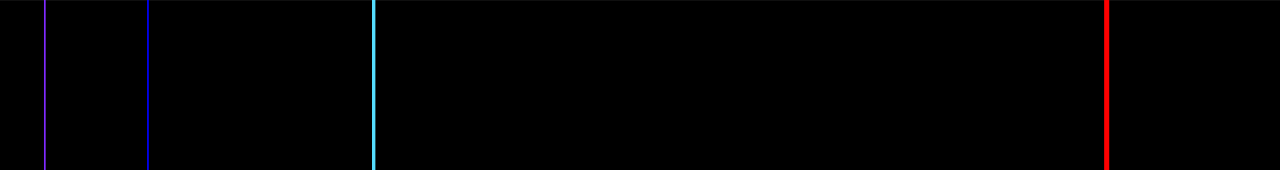
\includegraphics[width=0.70\linewidth]{images/book3/hydrogen-emission-spectrum.png}

{\small 氢的可见发射光谱：巴耳末线位于 \qty{656}{nm}、\qty{486}{nm}、\qty{434}{nm} 和 \qty{410}{nm}，每条都对应跃迁到 $n = 2$ 的能级。}
\end{omfigure}

\begin{omfigure}
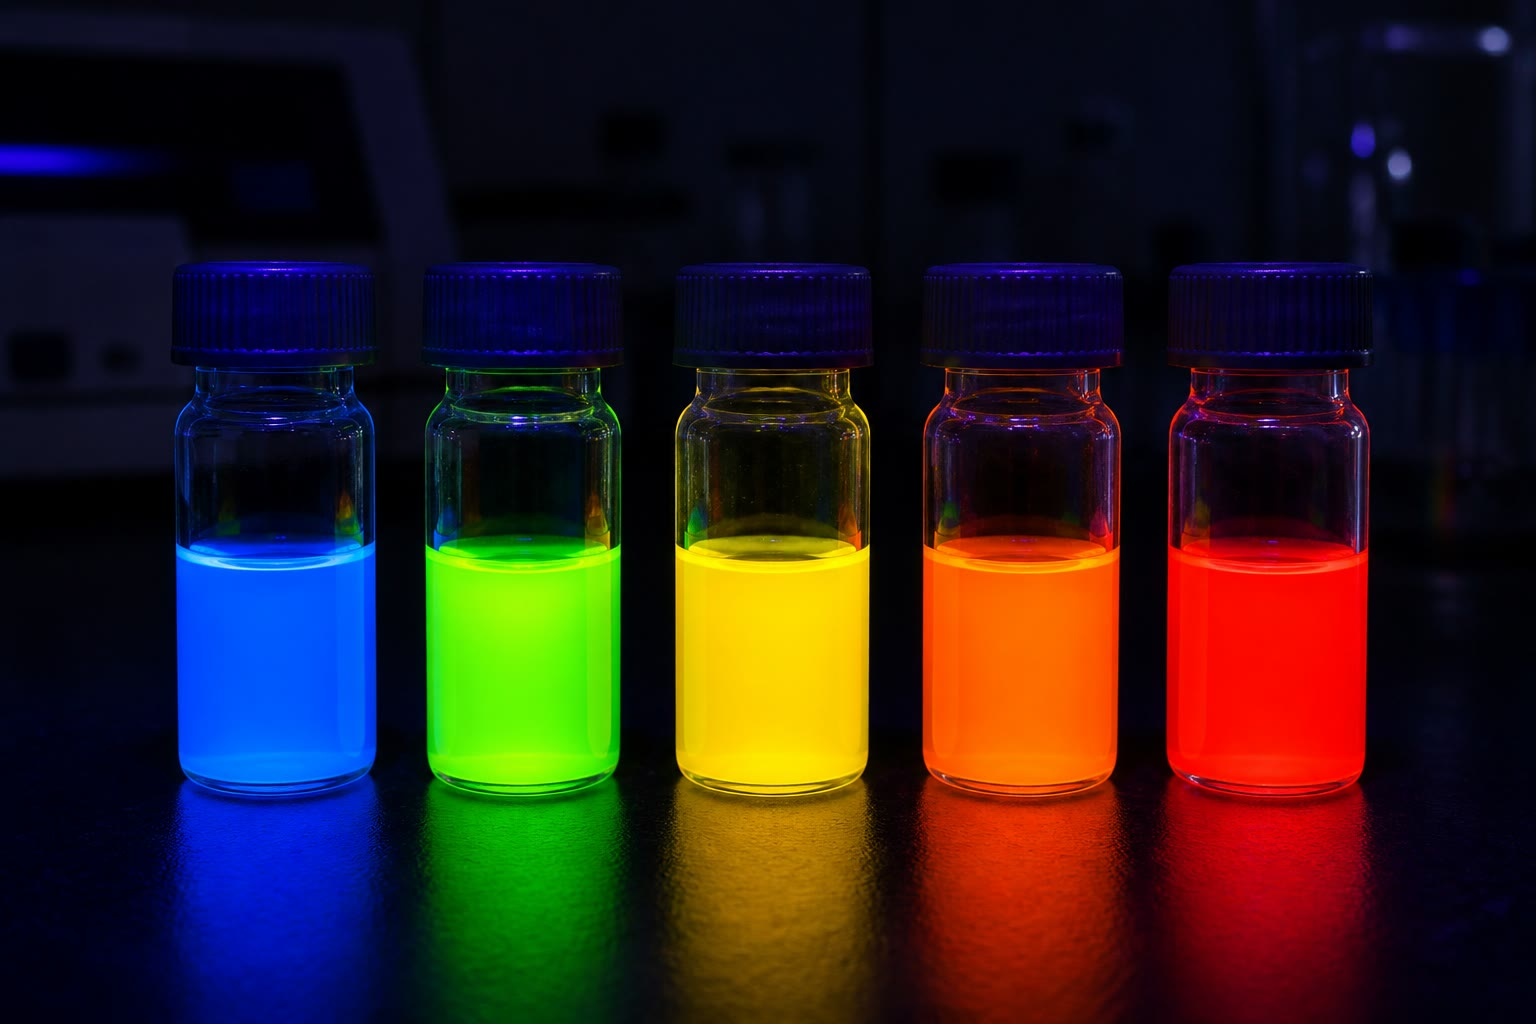
\includegraphics[width=0.60\linewidth]{images/book3/ai/b3-30-quantum-dots-vials.jpg}

{\small 同一材料的\omterm{ex:b1:quantum-introduction:dot}{量子点}装在小瓶中：纳米晶体越小，限制能越大，光越偏蓝——颜色由尺寸决定。}
\end{omfigure}

\section{问题：氢谱与量子点}

\begin{problem}[{周末问题——用光与电压表测量 $h$，
由三个常量构造氢原子，
并由尺寸选择晶体的颜色}]
\label{pb:b1:quantum-introduction:1}
常量：$h = \qty{6.626e-34}{J.s}$，$\hbar = \qty{1.055e-34}{J.s}$，$c =
\qty{3.00e8}{m/s}$，$e = \qty{1.602e-19}{C}$，$m_e = \qty{9.11e-31}{kg}$，
$1/4\pi\varepsilon_0 = \qty{8.99e9}{SI}$，$hc = \qty{1240}{eV.nm}$。

\medskip
\noindent\textbf{第一部分——测量\omterm{thm:b1:quantum-introduction:photon}{普朗克常量}。}
用单色光照射钾光电阴极，
测得\omterm{prop:b1:quantum-introduction:photoelectric}{遏止电压}：在 \qty{6.0e14}{Hz} 时为 \qty{0.30}{V}，
在 \qty{7.0e14}{Hz} 时为 \qty{0.69}{V}，在 \qty{8.0e14}{Hz} 时为 \qty{1.13}{V}，
在 \qty{9.0e14}{Hz} 时为 \qty{1.50}{V}，在 \qty{1.1e15}{Hz} 时为 \qty{2.36}{V}。
\begin{enumerate}
  \item 描述该光电管，解释反向\omterm{def:b1:dc-circuits:voltage}{电压}为何能阻止电流，
        以及 $eV_s$ 测量的是什么。
  \item 写出爱因斯坦关系式，并说明 $V_s(\nu)$ 的斜率与
        截距分别给出什么。
  \item 由数据（作线性拟合，或取两个极端点）推出 $h$，
        并与公认值比较。
  \item 求钾的\omterm{prop:b1:quantum-introduction:photoelectric}{逸出功}（以 eV 计）；求\omterm{def:b1:filters-transfer-functions:bode}{截止频率}与波长；
        红色激光笔能否打出电子？
  \item 灯的光强加倍：$V_s$ 与电流各有何变化？
        为何这与纯波动图像不相容？
  \item 经典估算：一束 \qty{1}{\micro W/m^2} 的光照在金属上；
        一个原子约提供 \qty{1e-20}{m^2} 的面积：
        要在一个原子上积累 \qty{2.2}{eV}，需要多长时间？
        实际观察到的又是什么？
\end{enumerate}

\medskip
\noindent\textbf{第二部分——玻尔\omterm{prop:b1:quantum-introduction:hydrogen}{氢原子}。}
\begin{enumerate}[resume]
  \item 电子在绕固定质子的半径为 $r$ 的\omterm{prop:b1:central-forces:effective}{圆轨道}上运动：
        求速率 $v(r)$ 与\omterm{thm:b1:work-and-energy:em}{机械能} $E(r)$。
  \item 玻尔条件 $m_evr = n\hbar$：证明 $r_n = n^2a_0$，
        并数值给出 $a_0 = 4\pi\varepsilon_0\hbar^2/m_ee^2$。
  \item $E_n = E_1/n^2$，其中 $E_1 = -m_ee^4/[2(4\pi\varepsilon_0)^2\hbar^2]$；
        以 eV 给出数值。
  \item 第一轨道上的速率及比值 $v_1/c$
        （精细结构常数 $\alpha \approx 1/137$）。
  \item 求谱线 $2 \to 1$（莱曼 $\alpha$）、$3 \to 2$
        与 $4 \to 2$（巴耳末 H$\alpha$、H$\beta$）的波长：哪些是可见的？
  \item 证明 $1/\lambda = R_H(1/n^2 - 1/p^2)$，并计算里德伯常量 $R_H$；
        求最短的巴耳末波长。
  \item 求\omterm{prop:b1:quantum-introduction:hydrogen}{氢原子}从\omterm{prop:b1:quantum-introduction:box}{基态}电离所需的能量；
        求恰好使其电离的光子波长。
  \item 德布罗意：证明轨道 $n$ 的周长为 $n$ 个波长；
        玻尔条件即为\omterm{thm:b1:wave-propagation:standing}{驻波}条件。
  \item 指出该模型有两处错误、一处完全正确之处，
        并说明完整理论中取代轨道的是什么。
\end{enumerate}

\medskip
\noindent\textbf{第三部分——\omterm{ex:b1:quantum-introduction:dot}{量子点}。}
半径为 $R$ 的 CdSe 纳米晶体束缚一个受激电子
（有效质量 $m_e^\ast = 0.13\,m_e$）及其留下的空穴
（$m_h^\ast = 0.45\,m_e$）；二者在半径为 $R$ 的球中的限制能均为 $h^2/8m^\ast R^2$，
（在本阶段不加证明地承认）；体相 CdSe 的带隙为
$E_g = \qty{1.74}{eV}$。
\begin{enumerate}[resume]
  \item 由\omterm{thm:b1:wave-propagation:standing}{驻波}条件推导一维盒中粒子的能量
        $E_n = n^2h^2/8mL^2$，
        并评论其与球形公式的类比。
  \item 求电子与空穴的限制能，
        其中 $R = \qty{2.0}{nm}$。
  \item 求发射光子的能量与波长，其中 $R = \qty{2.0}{nm}$、
        \qty{3.0}{nm} 与 \qty{4.0}{nm}；并给出颜色。
  \item 用一句话解释为何较小的\omterm{ex:b1:quantum-introduction:dot}{量子点}更偏蓝。
  \item 用不确定性原理检验\omterm{def:b1:units-dimensions:oom}{数量级}：
        以 $\Delta p \sim \hbar/R$ 估计 $R = \qty{2}{nm}$ 处电子的动量，
        并求其所蕴含的\omterm{thm:b1:work-and-energy:ke}{动能}。
  \item 某\omterm{ex:b1:quantum-introduction:dot}{量子点}在 \qty{577}{nm} 处发出 \qty{1.0}{nW}：求每秒光子数。
\end{enumerate}

\medskip
\noindent\textbf{第四部分——计数量子。}
\begin{enumerate}[resume]
  \item \qty{633}{nm} 处功率为 \qty{1.0}{mW} 的\omterm{rem:b1:quantum-introduction:rest}{激光器}每秒发出多少光子？
  \item 暗适应的\omterm{def:b1:optical-instruments:eye}{眼睛}探测到一次闪光，其中约有 $100$ 个 \qty{500}{nm} 的光子，
        在 \qty{0.1}{s} 内到达：求相应的功率。
  \item 一台调频天线在 \qty{100}{MHz} 处接收到 \qty{1.0}{pW}：求每秒光子数；
        有无可能逐个探测到它们？
  \item 总结：仅由 $h$、$e$、$m_e$ 出发，
        本题得到了原子世界的哪三个量，
        其量级各为多少？
\end{enumerate}
\end{problem}
